\section{问题二：全年逐日“计划—结算”两阶段模型}
\label{sec:q2}

\subsection{信息结构与我方预测模型}

问题二要求“在每天 0:00 制定当天的计划购电策略”，而 0:00 显然无法获得当日实测数据，
因此计划必须建立在\textbf{由历史实测（与 0:00 已发布的附件3 预报）构造的预测}之上，
当日实测数据只用于\textbf{结算}。结合第 3 节的周内规律（周五、周六用电低 36.8\%），
本文构造了一组\textbf{可分解、可堆叠}的预测模型，并用同一套因果管道逐项验证
（全部超参只在 1 月标定，2--12 月为外样本）。

\textbf{（1）负载预测：水平$\times$形状分解 + 分类组合}。记第 $d$ 天第 $t$ 时段负载为 $L_d(t)$。
把“日总量（水平）”与“日内曲线（形状）”分开建模：
\begin{equation}
L_d(t)=\underbrace{\Lambda_d}_{\text{水平}}\cdot\underbrace{\sigma_{c(d)}(t)}_{\text{形状}},\qquad
\Lambda_d=\frac{1}{4}\sum_{\tau\in H_d}\sum_{t}L_\tau(t),
\label{eq:basisL}
\end{equation}
其中 $H_d$ 为最近 4 个\textbf{同类日}（周五、周六记为“低”类 $c(d)=\text{L}$，其余五天记为“高”类），
$\sigma_{c}(t)$ 为同类日近 6 天归一化曲线（$L/\sum_tL$）的均值。
另构造\textbf{递推水平平滑}（对“昨日实际/预测总量比”做指数平滑，$\alpha=0.35$，限幅 $[0.85,1.15]$）
与\textbf{全局误差反馈}（近 3 日实测/预测比阻尼校正）两个候选，最后\textbf{按两类分别做凸组合}，
权重在 1 月标定集上网格搜索：
\begin{equation}
\hat L_d(t)=\sum_{k=1}^{4}w^{c(d)}_k\,g_k(t),\qquad
w^{\text{L}}=(0,\,0.3,\,0.7,\,0),\quad w^{\text{H}}=(0,\,1.0,\,0,\,0),
\label{eq:loadweights}
\end{equation}
即\textbf{周五/周六以“递推水平$\times$同类形状”为主（0.7），其余五天用“同类日水平$\times$形状”（1.0）}。
该结构使两类日子的误差同时下降（见 \cref{tab:fcacc}），这是“不分周五六的稳健统计”
（近 5 日中位数、近 5 日加权平均）误差高达 652$\sim$1056\,kW 的反证。

\textbf{（2）光伏预测：因果岭回归堆叠}。以 4 个基模型为输入：
近 4 日均值 $b_1$、误差反馈 $b_2$（近 2 日实测/预测比阻尼校正）、
LightGBM $b_3$（30 维特征：时段、星期、年内谐波、滞后与滚动的光伏/负载/电价、附件3 预报）、
以及\textbf{附件3 的 0:00 发布预报} $b_4$；用带时段与类别交互项的\textbf{岭回归}在历史样本上
（每 14 天用截至当时的样本重训，保证因果）学习最优权重：
\begin{equation}
\widehat{PV}_d(t)=\beta_0+\sum_{k=1}^{4}\beta_k\,b_k(t)+\beta_5\tau+\beta_6\mathbb{1}_{\text{L}}
+\beta_7\tau\mathbb{1}_{\text{L}},\qquad
\bm\beta=\arg\min_{\bm\beta}\sum_{j<d}\sum_t\Big(\sum_k\beta_kb_k^{(j)}(t)+\cdots-PV_j(t)\Big)^2+\alpha\|\bm\beta\|^2 .
\label{eq:basisPV}
\end{equation}
单模型都不如“近 4 日均值”（附件3 预报 206.7\,kW、晴空指数模型 213.3\,kW、
LightGBM 151.2\,kW、近 4 日均值 152.0\,kW），
但\textbf{堆叠后 MAE 降到 136.9\,kW（$-9.9\%$）}——收益来自多源信息的最优组合。

\textbf{（3）实时电价预测（用于第 \ref{sec:q4} 节的“未知电价”情形）}：
先取同类日近 6 天同槽位中位数作廓线、并按最近同类日水平做自适应缩放，
再与廓线误差反馈、LightGBM 做同样的因果岭回归堆叠，MAE 由同类日均价的 0.0581
降到 \textbf{0.0367 元/kWh}。

\begin{table}[htbp]
\centering
\caption{预测模型精度对照（2.1--12.31 外样本，单位：负荷/光伏 kW、电价 元/kWh）}
\label{tab:fcacc}
\scriptsize
\begin{tabular}{@{}llccc@{}}
\toprule
对象 & 模型 & MAE & RMSE & 日总量 MAPE \\
\midrule
\multirow{5}{*}{负载}
& 近 4 个同类日均值（原依据） & 137.52 & 191.59 & 1.06\% \\
& 指数加权同类日（8 日，0.85） & 140.45 & 196.61 & 1.36\% \\
& 相似日 kNN（5 个同类日） & 286.99 & 448.43 & 4.76\% \\
& 岭回归 / LightGBM（逐时段特征） & 188.58 / 159.32 & 283.72 / 259.71 & 2.77\% / 1.73\% \\
& \textbf{水平$\times$形状 + 分类凸组合（采用）} & \textbf{132.28} & \textbf{182.24} & \textbf{0.94\%} \\
\midrule
\multirow{5}{*}{光伏}
& 近 4 日均值（原依据） & 151.95 & 307.33 & 3.64\% \\
& 附件3 的 0:00 预报 & 206.65 & 388.78 & 5.27\% \\
& 晴空指数模型（近 10 日 $k\times$包络） & 213.33 & 384.00 & 3.53\% \\
& LightGBM（30 维特征） & 151.24 & 302.57 & 4.14\% \\
& \textbf{因果岭回归堆叠（采用）} & \textbf{136.85} & \textbf{261.74} & \textbf{3.49\%} \\
\midrule
\multirow{3}{*}{电价}
& 同类日近 30 日均价 & 0.0581 & --- & 1.75\% \\
& 廓线 + 自适应水平 / LightGBM & 0.0372 / 0.0370 & 0.052 / 0.053 & 1.75\% / 1.85\% \\
& \textbf{因果岭回归堆叠（采用）} & \textbf{0.0367} & \textbf{0.050} & 1.86\% \\
\midrule
\multicolumn{2}{@{}l}{负载分类精度（采用 vs 原依据）} & 周五六 142.21 / 154.60 & 其他五天 128.33 / 130.73 & 见正文 \\
\bottomrule
\end{tabular}
\end{table}

\textbf{（4）报童安全裕度}。定义净需求预测残差
$e_d(t)=\big(L_d(t)-\hat L_d(t)\big)-\big(PV_d(t)-\widehat{PV}_d(t)\big)$，
计划所用的“计划净需求”为预测加裕度：
\begin{equation}
\tilde N_d(t)=\hat L_d(t)-\widehat{PV}_d(t)+b_d(t),\qquad
b_d(t)=\mathrm{Quantile}_{q}\big(\{e_\tau(t)\}_{\tau\in\text{近30天}}\big).
\label{eq:buffer}
\end{equation}
分位水平 $q$ 由报童模型\cite{newsboy}确定：购电偏少的额外代价为紧急电价与基准电价之差 $c_u=5p-p=4p$，
购电偏多的代价为基准电价 $c_o=p$，故理论最优服务水平
\begin{equation}
q^*=\frac{c_u}{c_u+c_o}=\frac{4p}{4p+p}=0.8 .
\label{eq:newsboy}
\end{equation}
但由于日内实时平衡控制已能吸收大部分意外偏差，实测最优分位低于理论值：在 1 月标定集上
\begin{equation}
\mathrm{Cost}_{1\text{月}}(q=0.5/0.6/\textbf{0.7}/0.8/0.9)
=1\,282\,669\,/\,1\,244\,876\,/\,\bm{1\,237\,127}\,/\,1\,252\,414\,/\,1\,317\,816\ \text{元},
\label{eq:qtune}
\end{equation}
故取 $\bm{q^*=0.7}$，并在 2--12 月做外样本评估；储能放电下限取物理下限
$\underline E=1200$ kWh（第 \ref{sec:compare} 节给出裕度形式与分位水平的敏感性）。

\subsection{计划模型与结算模型（分开建模）}

\textbf{（1）0:00 计划模型}。以 $\tilde N_d$ 为输入求解式 \eqref{eq:obj}--\eqref{eq:c5}
（其中 $\hat L$ 替换为 $\hat L+b$、$\widehat{PV}$ 替换为预测值），得到计划购电量 $P^0_t$
与计划充放电量 $C^0_t,D^0_t$，并给出计划储电量轨迹 $E^0_t$。

\textbf{（2）日内结算模型：实时平衡控制}。计划报出后\textbf{购电量 $P^0_t$ 不再改变}
（否则等于允许“事后修改计划”），但储能是微网内部可控设备，题面又要求
“微网提供的电能不可低于小区负载”，因此运行中必须用储能\textbf{实时兜底}。
本文把这一过程写成\textbf{逐时段因果控制规则}：时段 $t$ 的决策只使用当前时刻可获得的量
（当前实测 $L_t,PV_t$、当前储电量 $E_t$ 与已锁定计划），\textbf{不使用任何未来实测}。

需要特别强调：\textbf{问题二只有 0:00 一个决策时刻}。上面这条规则并非“日内重新优化”，
而是与计划 $(P^0,C^0,D^0)$ \textbf{同时}在 0:00 就确定下来、并写入策略的一条\textbf{响应规则}
（式 \eqref{eq:clip}--\eqref{eq:socrec} 中不含任何未来信息，也不需要在线求解任何优化问题，
只是把偏差按“先动用计划充放电的可调空间、再动用储能存量、最后才紧急购电”的优先级消化）。
换言之，本文的 0:00 决策输出的是\textbf{“购电计划 $+$ 储能响应规则”这一对}
（相当于一个状态反馈策略 $\pi_t(\cdot)$），日内不产生任何新的、免费的调整机会；
若不采用该规则而僵硬照表执行（缺口一律按 $5p_t$ 紧急购电），全年费用将升至 14\,557\,730 元
（\cref{tab:q2exec}），这正是该规则的价值所在。

记 $\bar C=833.33$ kWh/10\,min（5000 kW）、$\eta_c=\eta_d=0.9$、
储电量上下限 $\underline{E}=1200,\ \overline{E}=10800$ kWh。控制规则为：

\textbf{① 可行性裁剪}：把计划充放电量裁剪到当前状态可达范围
\begin{equation}
C^{o}_t=\text{min}\Big\{\text{max}(C^0_t,0),\ \bar C,\ \frac{\overline{E}-E_t}{\eta_c}\Big\},\qquad
D^{o}_t=\text{min}\Big\{\text{max}(D^0_t,0),\ \bar C,\ \eta_d\big(E_t-\underline{E}+\eta_cC^{o}_t\big)\Big\}.
\label{eq:clip}
\end{equation}

\textbf{② 计划口径缺口}：$\Delta_t=L_t-\big(PV_t+P^0_t+D^{o}_t-C^{o}_t\big)$。
若 $\Delta_t>0$（实际比计划“更缺电”），先\textbf{少充}、再\textbf{多放}：
\begin{align}
C_t&=\text{max}\big(0,\ C^{o}_t-\Delta_t\big),\qquad
\Delta'_t=\text{max}\big(0,\ \Delta_t-C^{o}_t\big),\label{eq:up1}\\
D_t&=D^{o}_t+\text{min}\Big\{\Delta'_t,\ \bar C-D^{o}_t,\ \eta_d\big(E_t-\underline{E}+\eta_cC_t\big)-D^{o}_t\Big\},\qquad
E^{\text{急}}_t=\text{max}\big(0,\ \Delta'_t-(D_t-D^{o}_t)\big).\label{eq:up2}
\end{align}
即\textbf{先动用计划充放电的可调空间，再动用储能存量}；仍兜不住的缺口
$E^{\text{急}}_t$ 只能按 $5p_t$ 紧急购电。

\textbf{③ 计划口径富余}：若 $\Delta_t<0$，先\textbf{少放}、再\textbf{多充}：
\begin{align}
D_t&=\text{max}\big(0,\ D^{o}_t+\Delta_t\big),\qquad
\Delta''_t=\text{min}\big(0,\ \Delta_t+D^{o}_t\big),\label{eq:dn1}\\
C_t&=C^{o}_t+\text{min}\Big\{-\Delta''_t,\ \bar C-C^{o}_t,\
\frac{\overline{E}-E_t+D_t/\eta_d}{\eta_c}-C^{o}_t\Big\},\label{eq:dn2}
\end{align}
剩余富余 $\big(-\Delta''_t-(C_t-C^{o}_t)\big)$ 由\textbf{弃光}吸收（题面允许光伏未上网部分直接丢弃）。

最后按
\begin{equation}
E_{t+1}=E_t+\eta_cC_t-\frac{D_t}{\eta_d}
\label{eq:socrec}
\end{equation}
递推储电量。可证式 \eqref{eq:clip}--\eqref{eq:socrec} 自动满足
$C_t,D_t\in[0,\bar C]$、$E_t\in[\underline E,\overline E]$ 与“不同时充放电”三项物理约束
（数值实现中亦以断言逐时段校验），且\textbf{所有量均为 $t$ 时刻已知}，故该规则是
\textbf{可实行的（online、因果）}。当日费用为
\begin{equation}
\text{Cost}_d=\sum_t p_tP^0_t+\sum_t 5p_tE^{\text{急}}_t ,
\label{eq:q2cost}
\end{equation}
储电量链条 $E_{145}^{(d)}=E_1^{(d+1)}$ 逐日递推，1 月为预热期，结果自 2 月 1 日起输出。

\textbf{（3）为什么“分开建模”是必要的}。若把两个阶段合并为一个“事后最优”模型
（用当日实测重新优化储能），等于允许 0:00 决策使用未来信息，得到的是\textbf{不可实行的}
下界而非策略。本文的“计划（历史信息）$+$ 实时平衡（当前信息）”结构下，
决策者的信息集随时间单调增长，不存在事后调整空间。
作为对照（\cref{tab:q2exec}）：若\textbf{僵硬执行}计划，全年费用升至 14\,557\,730 元；
实时平衡控制把它降到 \textbf{13\,655\,835 元（$-6.2\text{\%}$）}；
而“完美信息再调度”（不可实行）为 13\,368\,722 元。

\begin{table}[htbp]
\centering
\caption{问题二：同一计划下三种执行／结算方式的全年费用对照（2.1--12.31）}
\label{tab:q2exec}
\small
\begin{tabular}{@{}llccc@{}}
\toprule
执行方式 & 是否可实行 & 计划购电费(元) & 紧急购电费(元) & 总费用(元) \\
\midrule
僵硬执行计划（无日内平衡） & 可实行 & 12\,862\,043 & 1\,695\,687 & 14\,557\,730 \\
\textbf{实时平衡控制（采用）} & \textbf{可实行} & \textbf{12\,866\,999} & \textbf{788\,836} & \textbf{13\,655\,835} \\
完美信息再调度（事后最优） & 否（需未来实测） & 12\,866\,999 & 501\,723 & 13\,368\,722 \\
\bottomrule
\end{tabular}
\end{table}

\begin{figure}[htbp]
\centering
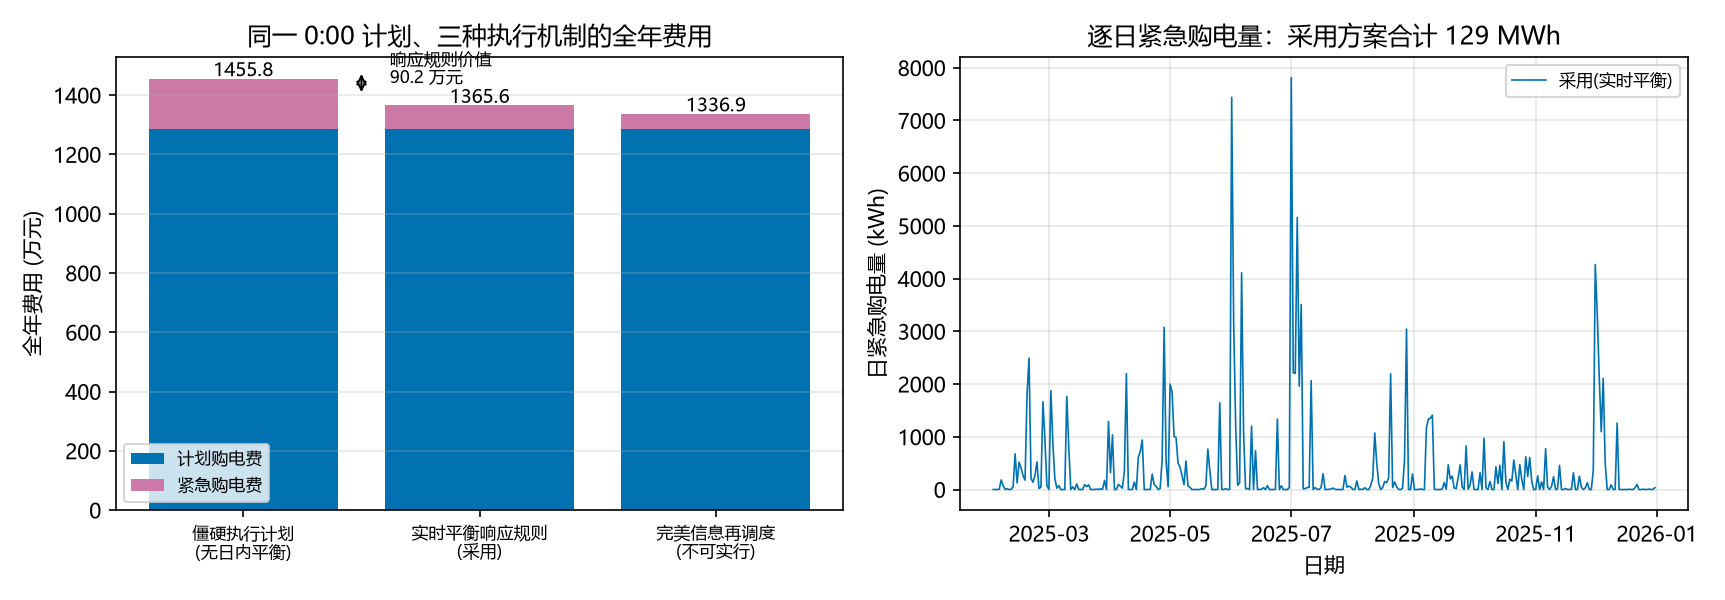
\includegraphics[width=0.95\textwidth]{figures/fig_q2_exec.png}
\caption{同一 0:00 计划下三种执行机制的全年费用分解（左）与采用方案的逐日紧急购电量（右）：
“0:00 定下的响应规则”把紧急购电费由 169.6 万元压到 78.9 万元}
\label{fig:q2exec}
\end{figure}

\subsection{全年结果}

\begin{table}[htbp]
\centering
\caption{问题二全年（2025-02-01 至 12-31，334 天）各方法对照
（全部方法采用同一实时平衡控制结算）}
\label{tab:q2cmp}
\scriptsize
\begin{tabular}{@{}lcccccl@{}}
\toprule
方法（0:00 计划依据） & 计划购电费(元) & 紧急购电费(元) & 总费用(元) & 紧急电量(kWh) & 相对采用 & 说明 \\
\midrule
\textbf{升级预测模型（采用）} & \textbf{12\,866\,999} & \textbf{788\,836} & \textbf{13\,655\,835} & \textbf{129\,289} & --- & 本文方法 \\
原依据（近 4 个同类日均值 $+$ 近 4 日光伏） & 12\,932\,582 & 915\,601 & 13\,848\,183 & 150\,493 & $+1.41\text{\%}$ & 仅换预测依据 \\
附件1 典型日曲线 + 报童 $q=0.7$ & 14\,971\,784 & 3\,346\,902 & 18\,318\,686 & 546\,489 & $+34.1\text{\%}$ & 忽略日际变化 \\
无储能（升级预测+报童） & 18\,155\,061 & （含于左） & 18\,155\,061 & --- & $+32.9\text{\%}$ & 储能价值对照 \\
昨日外推 + 报童 $q=0.6$ & 12\,872\,034 & 8\,619\,722 & 21\,491\,755 & 1\,615\,300 & $+57.4\text{\%}$ & 仅用昨日信息 \\
昨日外推 + 报童 $q=0.8$ & 14\,456\,337 & 7\,333\,092 & 21\,789\,429 & 1\,350\,662 & $+59.6\text{\%}$ & 裕度过大 \\
昨日外推（无裕度） & 12\,296\,521 & 10\,219\,271 & 22\,515\,792 & 1\,887\,772 & $+64.9\text{\%}$ & 朴素外推 \\
两阶段随机规划 SAA（近 20 日情景） & 8\,752\,681 & 31\,201\,329 & 39\,954\,010 & 6\,928\,843 & $+192.6\text{\%}$ & 见第~\ref{sec:compare} 节失效分析 \\
完全信息下界（天眼链式） & 12\,286\,531 & 0 & 12\,286\,531 & 0 & $-10.0\text{\%}$ & 不可达下界 \\
\bottomrule
\end{tabular}
\end{table}

由\cref{tab:q2cmp} 可得三点结论：

\begin{enumerate}[label=(\arabic*), leftmargin=2.4em, itemsep=1pt]
\item \textbf{预测模型的精度是本题最大的杠杆}：把“昨日外推”升级为“水平$\times$形状分解 +
分类组合 + 光伏堆叠”，全年费用由 21\,491\,755 元降至 \textbf{13\,655\,835 元（下降 36.5\%）}，
紧急购电量由 1.62 GWh 降至 0.13 GWh；负载预测 MAE 由 650.0 kW 降到 132.3 kW（$-79.6\text{\%}$），
光伏 MAE 由 307.3（RMSE）对应的 152.0 kW 降到 136.9 kW。
\item \textbf{报童裕度必须与预测依据联合标定}：裕度形式（净残差经验分位 / 正态参数化 /
分噪声叠加 / 60--90 天长窗）差异在 $-0.5\%\sim+0.6\%$ 之间，
而\textbf{分位水平}偏离 0.7 的代价大得多（$q=0.5$ 时 $+8.3\text{\%}$，\cref{tab:sens}）。
\item \textbf{储能价值显著}：无储能时全年 18\,155\,061 元，储能可节约
\textbf{449.9 万元（24.8\%）}；距完全信息下界 136.9 万元，
说明本文方法已接近该信息结构下的效率前沿。
\end{enumerate}

\begin{figure}[htbp]
\centering
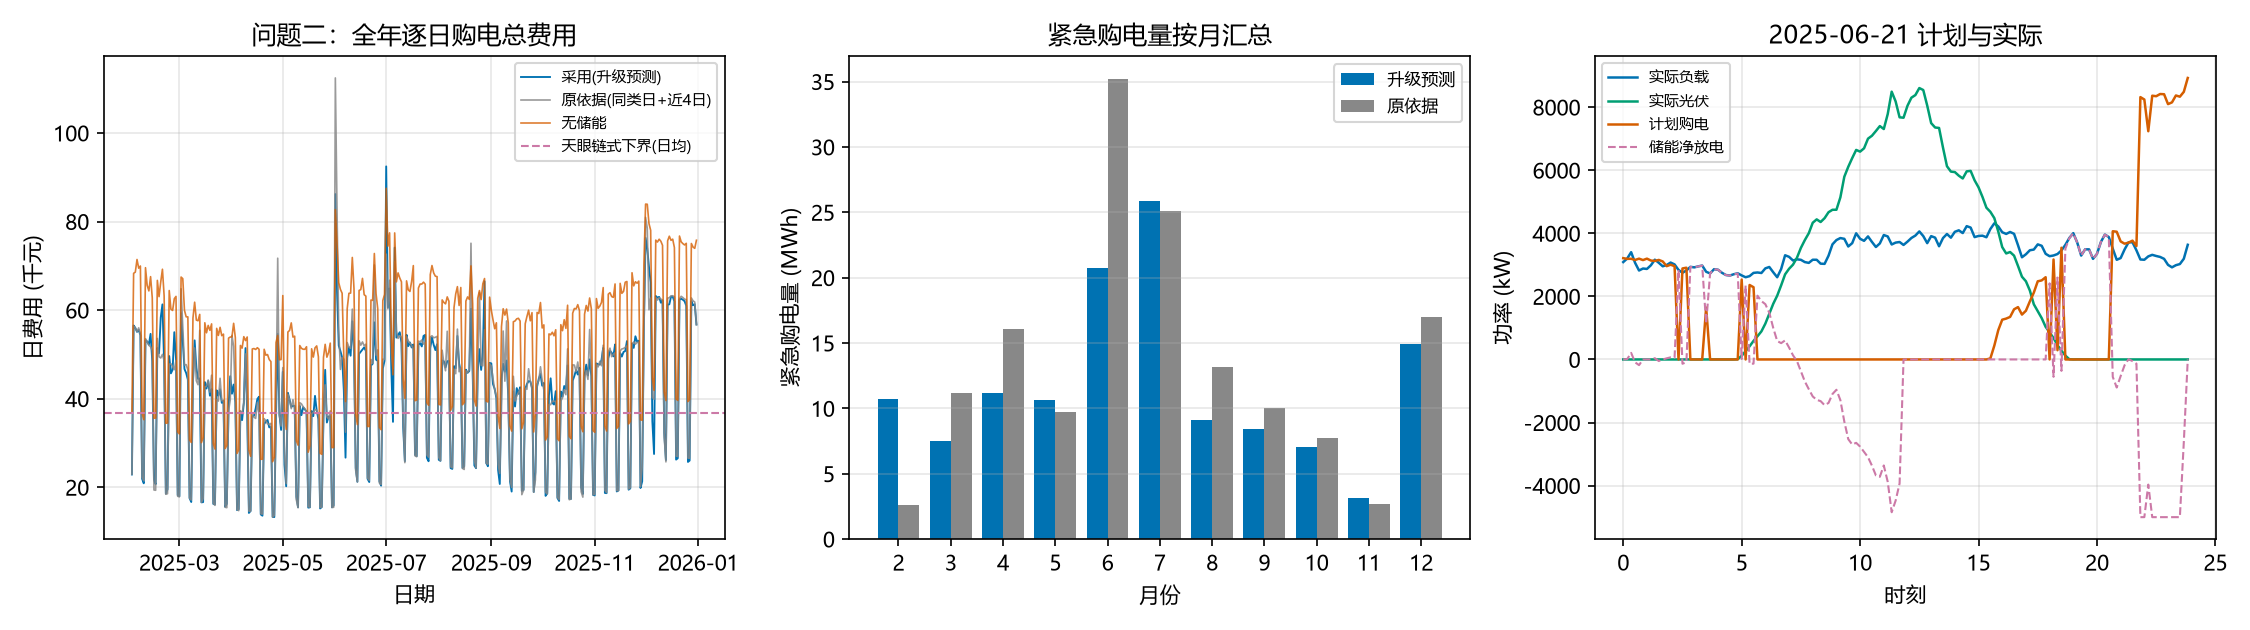
\includegraphics[width=0.95\textwidth]{figures/fig_q2_annual.png}
\caption{问题二：全年逐日购电总费用对比（左）、紧急购电量按月汇总（中）、
2025-06-21 计划与实际（右）}
\label{fig:q2}
\end{figure}

\begin{figure}[htbp]
\centering
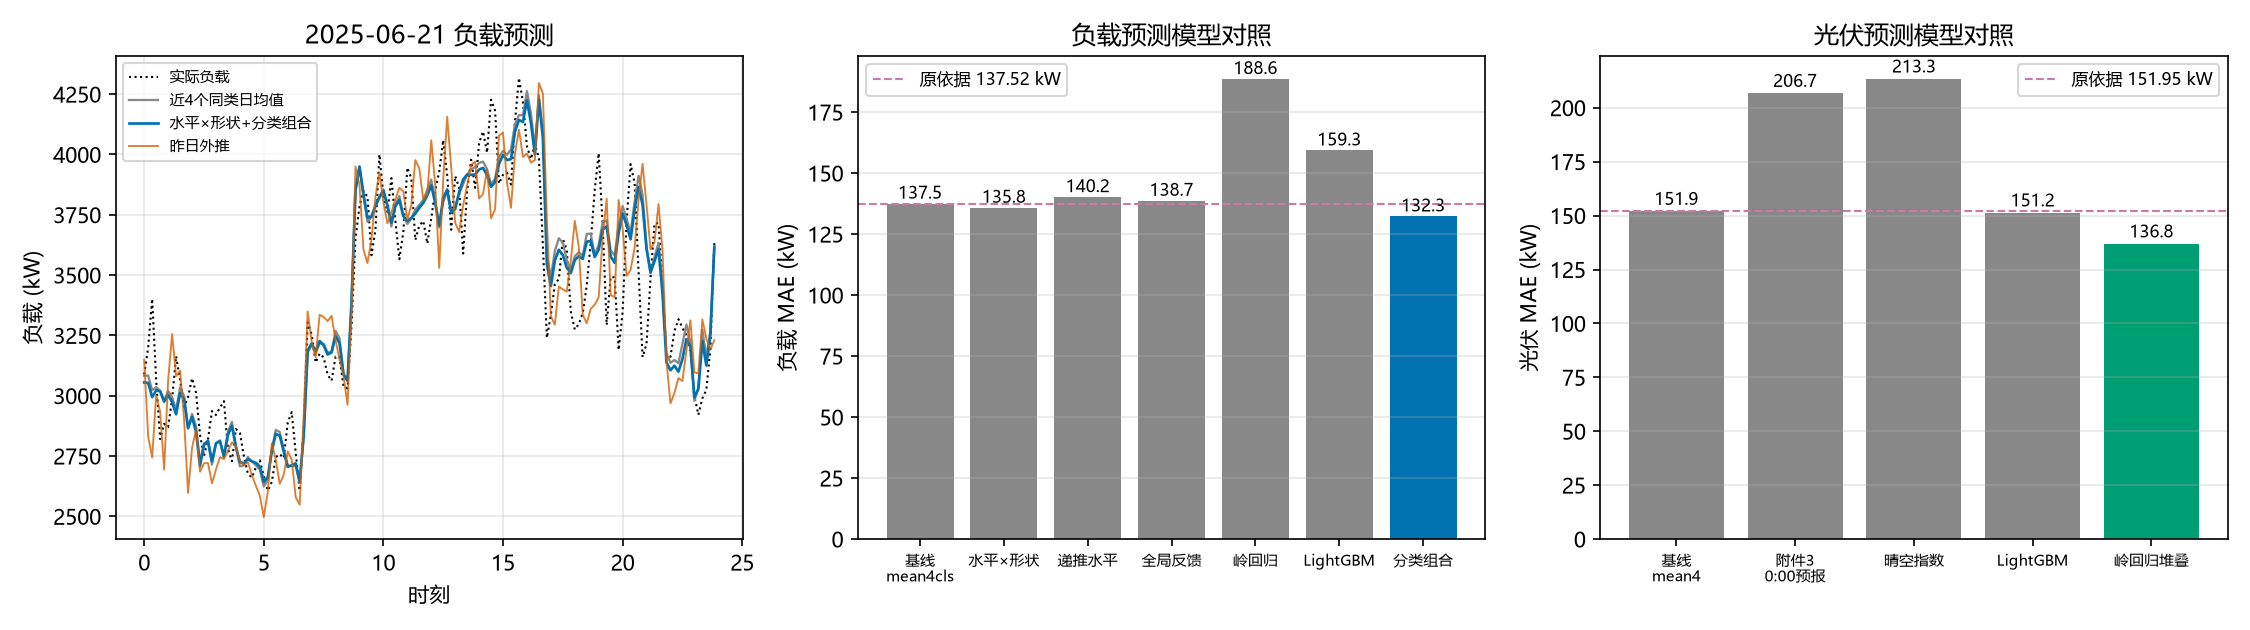
\includegraphics[width=0.62\textwidth]{figures/fig_q2_basis.png}
\caption{预测模型对照：分类组合负荷模型与岭回归堆叠光伏模型的精度优势}
\label{fig:q2basis}
\end{figure}

\begin{figure}[htbp]
\centering
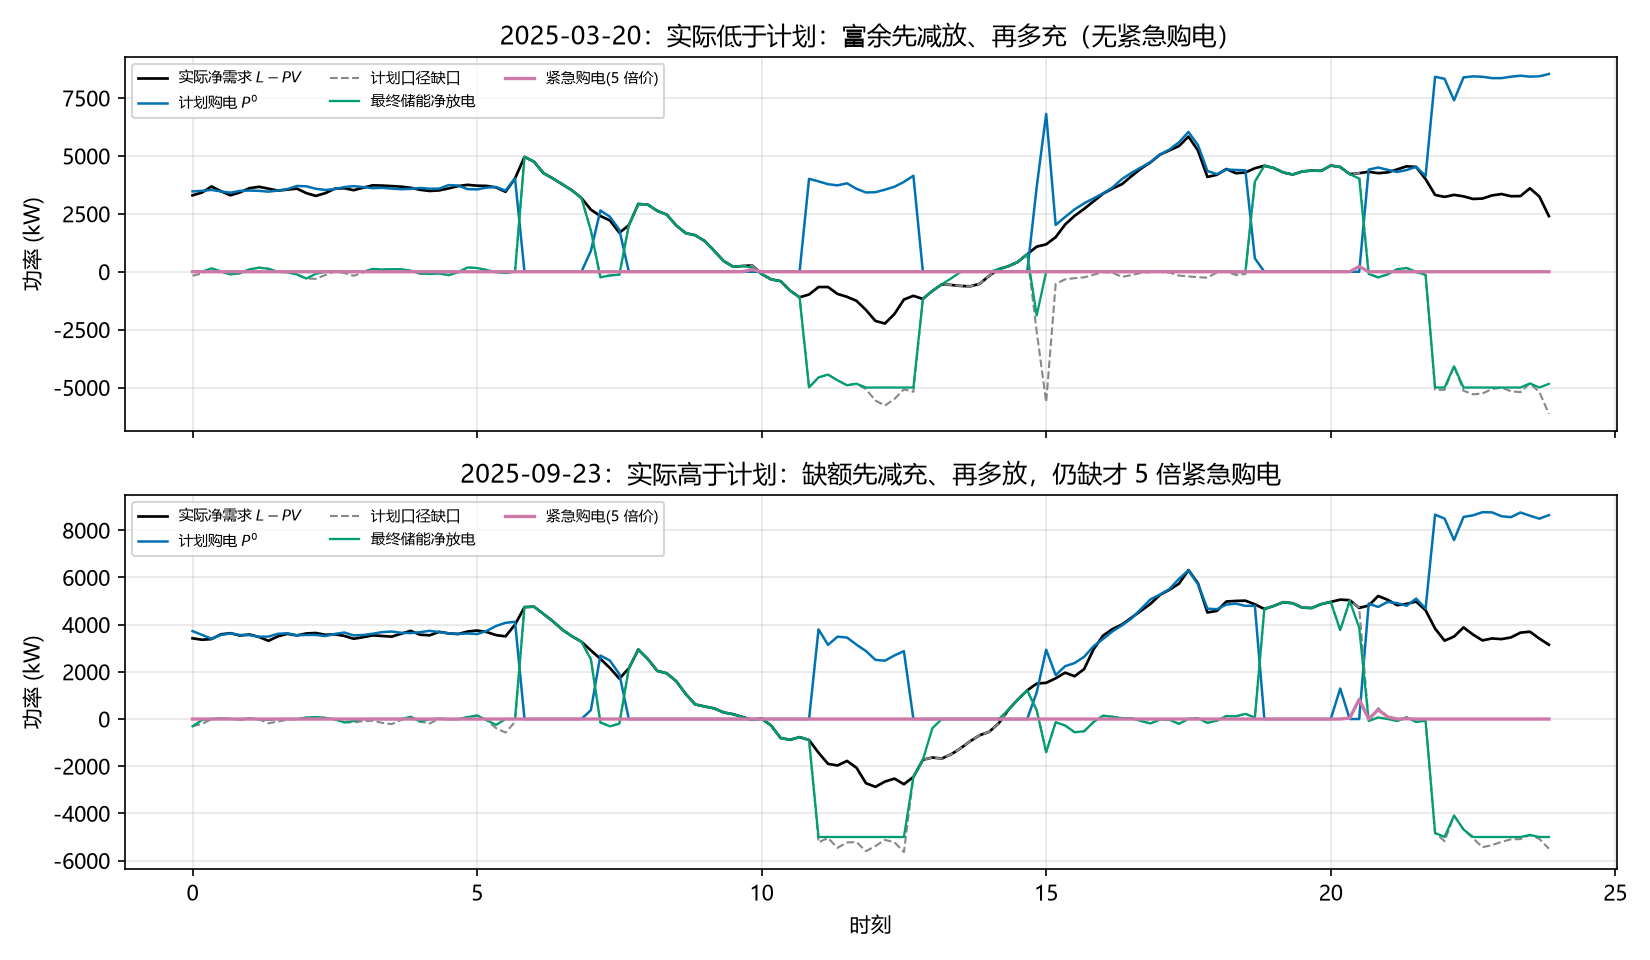
\includegraphics[width=0.95\textwidth]{figures/fig_q2_balance.png}
\caption{实时平衡控制过程：上行（03-20）计划偏保守、储能吸收富余；下行（09-23）实际高于计划、
储能兜底后仍有少量紧急购电}
\label{fig:q2balance}
\end{figure}

\subsection{指定日期结果（表 1、表 2、表 3 格式）}

\begin{table}[htbp]
\centering
\caption{问题二：指定日期关键时段计划购电量与全天购电量、购电费（表 1 格式，kWh/元）}
\label{tab:q2t1}
\scriptsize
\begin{tabular}{@{}lcccc@{}}
\toprule
时间段 & 2025-03-20 & 2025-06-21 & 2025-09-23 & 2025-12-21 \\
\midrule
10:00--10:10 & 0.00 & 0.00 & 0.00 & 0.00 \\
12:00--12:10 & 572.73 & 0.00 & 417.97 & 970.56 \\
14:00--14:10 & 0.00 & 0.00 & 0.00 & 0.00 \\
16:00--16:10 & 564.40 & 210.12 & 565.82 & 847.33 \\
18:00--18:10 & 702.62 & 0.00 & 775.60 & 716.85 \\
20:00--20:10 & 0.00 & 0.00 & 0.00 & 0.00 \\
\midrule
全天购电量 & 69\,247.84 & 37\,122.93 & 68\,471.78 & 97\,053.33 \\
全天购电费 & 41\,846.37 & 21\,173.98 & 42\,566.71 & 62\,140.33 \\
\bottomrule
\end{tabular}
\end{table}

\begin{table}[htbp]
\centering
\caption{问题二：指定日期最终储能充放电量与 0:00、24:00 储电量（表 2 格式，kWh）}
\label{tab:q2t2}
\scriptsize
\begin{tabular}{@{}lcccccccc@{}}
\toprule
\multirow{2}{*}{时间段} & \multicolumn{2}{c}{2025-03-20} & \multicolumn{2}{c}{2025-06-21} &
\multicolumn{2}{c}{2025-09-23} & \multicolumn{2}{c}{2025-12-21} \\
\cmidrule(lr){2-3}\cmidrule(lr){4-5}\cmidrule(lr){6-7}\cmidrule(lr){8-9}
& 充电 & 放电 & 充电 & 放电 & 充电 & 放电 & 充电 & 放电 \\
\midrule
0:00--4:00 & 120.41 & 177.57 & 90.73 & 3628.48 & 110.84 & 58.65 & 72.60 & 100.04 \\
4:00--8:00 & 169.32 & 5935.75 & 389.36 & 4839.09 & 178.05 & 6091.11 & 854.59 & 1456.11 \\
8:00--12:00 & 6028.92 & 2761.36 & 9973.71 & 0.00 & 5607.93 & 1896.62 & 5592.70 & 7159.56 \\
12:00--16:00 & 4952.21 & 254.72 & 0.00 & 0.00 & 4598.44 & 465.74 & 7080.82 & 2300.86 \\
16:00--20:00 & 4.10 & 5751.77 & 151.96 & 5590.59 & 125.58 & 5749.56 & 4.34 & 5832.12 \\
20:00--24:00 & 10\,722.55 & 2936.83 & 9820.78 & 2487.33 & 10\,646.53 & 2956.95 & 10\,666.67 & 2811.39 \\
\midrule
0:00 储电量 & \multicolumn{2}{c}{10\,800.00} & \multicolumn{2}{c}{10\,800.00} &
\multicolumn{2}{c}{10\,747.68} & \multicolumn{2}{c}{10\,800.00} \\
24:00 储电量 & \multicolumn{2}{c}{10\,800.00} & \multicolumn{2}{c}{10\,800.00} &
\multicolumn{2}{c}{10\,756.51} & \multicolumn{2}{c}{10\,800.00} \\
\bottomrule
\end{tabular}
\end{table}

\begin{table}[htbp]
\centering
\caption{问题二：指定日期紧急购电时间段与购电量（表 3 格式，kWh）}
\label{tab:q2t3}
\scriptsize
\begin{tabular}{@{}llll@{}}
\toprule
2025-03-20（合计 54.68） & 2025-06-21 & 2025-09-23（合计 228.74） & 2025-12-21（合计 31.13） \\
\midrule
9:50--10:00\ 16.02 & \multicolumn{1}{c}{无紧急购电} & 20:20--20:40\ 145.79 & 20:30--20:40\ 31.13 \\
20:30--20:40\ 38.66 & & 20:50--21:10\ 81.13 & \\
 & & 21:20--21:30\ 1.82 & \\
\bottomrule
\end{tabular}
\end{table}

四个指定日期的结果体现了“升级预测 + 报童裕度 + 实时平衡”的效果：6 月 21 日（周六，低负荷低价日）
计划量小而紧急购电为零；其余三日的紧急购电合计均不足 230 kWh，占全天购电量不足 0.35\%——
相较于原依据（\cref{tab:q2t3} 同类日期曾达 783.90 kWh）明显下降，
说明\textbf{预测精度提升直接转化为紧急购电量的下降}。
